The following section describes how the tests were set up and carried out.

\subsubsection{Experimental Setup}
The tests were carried out using an optical bench to guarantee more scientific accuracy. The experimental setup contained an optical bench, with a screen holder at the zero point where the QR code was positioned. The device currently being tested, Google Glass or smartphone, was then positioned at the specified mark on the optical bench using a clamp and pointed towards the QR code. See Figure~\ref{experimentalSetup} for a better understanding of the experimental setup. 

	\begin{figure}[ht!]
		\centering
		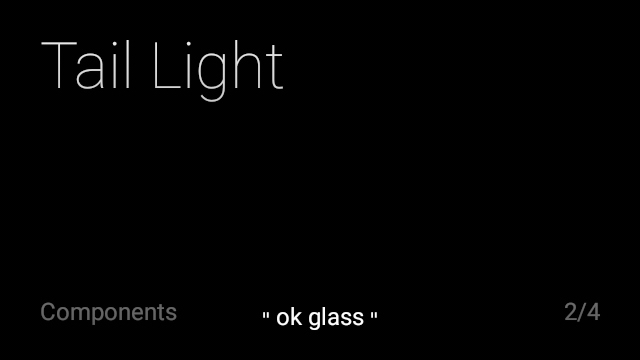
\includegraphics[width=110mm]{images/demo/componentText}
		\caption{todo change image The experimental setup.}
		\label{experimentalSetup}
	\end{figure}

In order to measure the time needed for the results of each test a specific class was built, called \texttt{Timer} and seen in Listing~\ref{timerClass}. The \texttt{Timer} class was built using the singleton design pattern. A singleton class is a class that can only be instanced once during the entire execution of an application, however the instance lives throughout the entire execution and may be accessed from anywhere in the application.

Using this pattern meant that the timer could be started in one class, and stop in another without having to pass the instance around, which potentially could affect performance.

\begin{lstlisting}[language=Java, caption={The Timer class}, label=timerClass]

public class Timer {
	private static Timer ourInstance = new Timer();
	public static Timer getInstance() { return ourInstance; }
	private Timer() {  }
	
	private boolean timerRunning = false;
	private Long startTime;
	private Long stopTime;
	
	public void startTimer() { 
		if(timerRunning) { Log.d("TIMER", "Timer already running"); }
		else 	{ startIme = System.nanoTime(); }
	}
	
	public void stopTimer() {
		if(!timerRunning) { Log.d("TIMER", "No timer running"); }
		else { stopTime = System.nanoTime()); }
	}
	
	private long getElapsedTime(int timerID) { return stopTime - startTime; }
	
	public void logElapsedTime(String information) {
		Log.d("TIMER", information + ": " + String.valueOf(getElapsedTime() + " nano seconds");
	}
}

\end{lstlisting}

\subsubsection{Text Length}
\begin{lstlisting}[language=Java, caption={The randomizer class}, label=todo]
private double randfrom(double min, double max)
{
	Random rand = new Random();
	double range = (max - min);
	return min + range * rand.nextDouble();
}

private String getChar(int pos, double rand)
{
	if(rand <= doubleList.get(pos) || pos+1 <= alph.size())
		return alph.get(pos);
		
	return getChar(pos+1, rand);
}

public String randchar()
{
	double rand = randfrom(0, 1);
	return getChar(0, rand);
}
\end{lstlisting}

\subsubsection{Distance to the QR Code}

	\begin{table}[ht!]
    		\caption{Average time of registering a QR code with varying distance.} \label{tab:distanceAverage}
		\centering \begin{tabularx}{\textwidth}{l|X|X|X} \hline
		\textbf{Distance (dm)} & \textbf{Google Glass} & \textbf{Samsung Galaxy SII} & \textbf{Samsung Galaxy SIII} \\ \hline \hline
       
		1	&	&	&	\\ \hline
		2	&	&	&	\\ \hline
		3	&	&	&	\\ \hline
		
		\end{tabularx}
	\end{table}

\subsubsection{Complexity of the QR Code}

	\begin{table}[H]%ht!]
    		\caption{Average time of registering a QR code with varying density.} \label{tab:complexityAverage}
		\centering \begin{tabularx}{\textwidth}{l|X|X|X} \hline
		\textbf{Encoded Characters} & \textbf{Google Glass} & \textbf{Samsung Galaxy SII} & \textbf{Samsung Galaxy SIII} \\ \hline \hline
       
		1	&	&	&	\\ \hline
		50	&	&	&	\\ \hline
		100	&	&	&	\\ \hline
		
		\end{tabularx}
	\end{table}

\subsubsection{Display Time}

	\begin{table}[ht!]
    		\caption{Average display time for Google Glass with varying information size.} \label{tab:averageDisplaySpeedGoogleGlass}
		\centering \begin{tabularx}{\textwidth}{l|X|X|X} \hline
		\textbf{Information Size (Byte)} & \textbf{Google Glass (ms)}  & \textbf{Samsung Galaxy SII (ms)}  & \textbf{Samsung Galaxy SIII (ms)} \\ \hline \hline
       
		100 k	&	&	&	 \\ \hline
		1 M		&	&	&	 \\ \hline
		10 M		&	&	&	 \\ \hline

		\end{tabularx}
	\end{table}